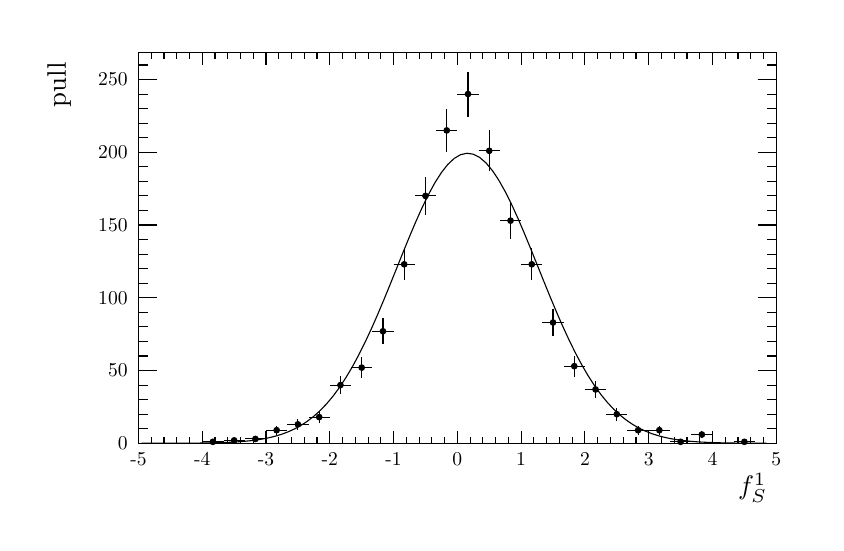
\begin{tikzpicture}
\pgfdeclareplotmark{cross} {
\pgfpathmoveto{\pgfpoint{-0.3\pgfplotmarksize}{\pgfplotmarksize}}
\pgfpathlineto{\pgfpoint{+0.3\pgfplotmarksize}{\pgfplotmarksize}}
\pgfpathlineto{\pgfpoint{+0.3\pgfplotmarksize}{0.3\pgfplotmarksize}}
\pgfpathlineto{\pgfpoint{+1\pgfplotmarksize}{0.3\pgfplotmarksize}}
\pgfpathlineto{\pgfpoint{+1\pgfplotmarksize}{-0.3\pgfplotmarksize}}
\pgfpathlineto{\pgfpoint{+0.3\pgfplotmarksize}{-0.3\pgfplotmarksize}}
\pgfpathlineto{\pgfpoint{+0.3\pgfplotmarksize}{-1.\pgfplotmarksize}}
\pgfpathlineto{\pgfpoint{-0.3\pgfplotmarksize}{-1.\pgfplotmarksize}}
\pgfpathlineto{\pgfpoint{-0.3\pgfplotmarksize}{-0.3\pgfplotmarksize}}
\pgfpathlineto{\pgfpoint{-1.\pgfplotmarksize}{-0.3\pgfplotmarksize}}
\pgfpathlineto{\pgfpoint{-1.\pgfplotmarksize}{0.3\pgfplotmarksize}}
\pgfpathlineto{\pgfpoint{-0.3\pgfplotmarksize}{0.3\pgfplotmarksize}}
\pgfpathclose
\pgfusepathqstroke
}
\pgfdeclareplotmark{cross*} {
\pgfpathmoveto{\pgfpoint{-0.3\pgfplotmarksize}{\pgfplotmarksize}}
\pgfpathlineto{\pgfpoint{+0.3\pgfplotmarksize}{\pgfplotmarksize}}
\pgfpathlineto{\pgfpoint{+0.3\pgfplotmarksize}{0.3\pgfplotmarksize}}
\pgfpathlineto{\pgfpoint{+1\pgfplotmarksize}{0.3\pgfplotmarksize}}
\pgfpathlineto{\pgfpoint{+1\pgfplotmarksize}{-0.3\pgfplotmarksize}}
\pgfpathlineto{\pgfpoint{+0.3\pgfplotmarksize}{-0.3\pgfplotmarksize}}
\pgfpathlineto{\pgfpoint{+0.3\pgfplotmarksize}{-1.\pgfplotmarksize}}
\pgfpathlineto{\pgfpoint{-0.3\pgfplotmarksize}{-1.\pgfplotmarksize}}
\pgfpathlineto{\pgfpoint{-0.3\pgfplotmarksize}{-0.3\pgfplotmarksize}}
\pgfpathlineto{\pgfpoint{-1.\pgfplotmarksize}{-0.3\pgfplotmarksize}}
\pgfpathlineto{\pgfpoint{-1.\pgfplotmarksize}{0.3\pgfplotmarksize}}
\pgfpathlineto{\pgfpoint{-0.3\pgfplotmarksize}{0.3\pgfplotmarksize}}
\pgfpathclose
\pgfusepathqfillstroke
}
\pgfdeclareplotmark{newstar} {
\pgfpathmoveto{\pgfqpoint{0pt}{\pgfplotmarksize}}
\pgfpathlineto{\pgfqpointpolar{44}{0.5\pgfplotmarksize}}
\pgfpathlineto{\pgfqpointpolar{18}{\pgfplotmarksize}}
\pgfpathlineto{\pgfqpointpolar{-20}{0.5\pgfplotmarksize}}
\pgfpathlineto{\pgfqpointpolar{-54}{\pgfplotmarksize}}
\pgfpathlineto{\pgfqpointpolar{-90}{0.5\pgfplotmarksize}}
\pgfpathlineto{\pgfqpointpolar{234}{\pgfplotmarksize}}
\pgfpathlineto{\pgfqpointpolar{198}{0.5\pgfplotmarksize}}
\pgfpathlineto{\pgfqpointpolar{162}{\pgfplotmarksize}}
\pgfpathlineto{\pgfqpointpolar{134}{0.5\pgfplotmarksize}}
\pgfpathclose
\pgfusepathqstroke
}
\pgfdeclareplotmark{newstar*} {
\pgfpathmoveto{\pgfqpoint{0pt}{\pgfplotmarksize}}
\pgfpathlineto{\pgfqpointpolar{44}{0.5\pgfplotmarksize}}
\pgfpathlineto{\pgfqpointpolar{18}{\pgfplotmarksize}}
\pgfpathlineto{\pgfqpointpolar{-20}{0.5\pgfplotmarksize}}
\pgfpathlineto{\pgfqpointpolar{-54}{\pgfplotmarksize}}
\pgfpathlineto{\pgfqpointpolar{-90}{0.5\pgfplotmarksize}}
\pgfpathlineto{\pgfqpointpolar{234}{\pgfplotmarksize}}
\pgfpathlineto{\pgfqpointpolar{198}{0.5\pgfplotmarksize}}
\pgfpathlineto{\pgfqpointpolar{162}{\pgfplotmarksize}}
\pgfpathlineto{\pgfqpointpolar{134}{0.5\pgfplotmarksize}}
\pgfpathclose
\pgfusepathqfillstroke
}
\definecolor{c}{rgb}{1,1,1};
\draw [color=c, fill=c] (0,0) rectangle (10,6.27517);
\draw [color=c, fill=c] (1.4,1.00403) rectangle (9.5,5.96141);
\definecolor{c}{rgb}{0,0,0};
\draw [c] (1.4,1.00403) -- (1.4,5.96141) -- (9.5,5.96141) -- (9.5,1.00403) -- (1.4,1.00403);
\draw [c] (2.345,1.00403) -- (2.345,1.02251);
\draw [c] (2.345,1.02251) -- (2.345,1.04099);
\draw [c] (2.21,1.02251) -- (2.345,1.02251);
\draw [c] (2.345,1.02251) -- (2.48,1.02251);
\foreach \P in {(2.345,1.02251)}{\draw[mark options={color=c,fill=c},mark size=2.402402pt,mark=*,mark size=1pt] plot coordinates {\P};}
\draw [c] (2.615,1.01485) -- (2.615,1.04099);
\draw [c] (2.615,1.04099) -- (2.615,1.06712);
\draw [c] (2.48,1.04099) -- (2.615,1.04099);
\draw [c] (2.615,1.04099) -- (2.75,1.04099);
\foreach \P in {(2.615,1.04099)}{\draw[mark options={color=c,fill=c},mark size=2.402402pt,mark=*,mark size=1pt] plot coordinates {\P};}
\draw [c] (2.885,1.02746) -- (2.885,1.05946);
\draw [c] (2.885,1.05946) -- (2.885,1.09147);
\draw [c] (2.75,1.05946) -- (2.885,1.05946);
\draw [c] (2.885,1.05946) -- (3.02,1.05946);
\foreach \P in {(2.885,1.05946)}{\draw[mark options={color=c,fill=c},mark size=2.402402pt,mark=*,mark size=1pt] plot coordinates {\P};}
\draw [c] (3.155,1.1149) -- (3.155,1.17034);
\draw [c] (3.155,1.17034) -- (3.155,1.22578);
\draw [c] (3.02,1.17034) -- (3.155,1.17034);
\draw [c] (3.155,1.17034) -- (3.29,1.17034);
\foreach \P in {(3.155,1.17034)}{\draw[mark options={color=c,fill=c},mark size=2.402402pt,mark=*,mark size=1pt] plot coordinates {\P};}
\draw [c] (3.425,1.17763) -- (3.425,1.24426);
\draw [c] (3.425,1.24426) -- (3.425,1.31089);
\draw [c] (3.29,1.24426) -- (3.425,1.24426);
\draw [c] (3.425,1.24426) -- (3.56,1.24426);
\foreach \P in {(3.425,1.24426)}{\draw[mark options={color=c,fill=c},mark size=2.402402pt,mark=*,mark size=1pt] plot coordinates {\P};}
\draw [c] (3.695,1.25825) -- (3.695,1.33665);
\draw [c] (3.695,1.33665) -- (3.695,1.41506);
\draw [c] (3.56,1.33665) -- (3.695,1.33665);
\draw [c] (3.695,1.33665) -- (3.83,1.33665);
\foreach \P in {(3.695,1.33665)}{\draw[mark options={color=c,fill=c},mark size=2.402402pt,mark=*,mark size=1pt] plot coordinates {\P};}
\draw [c] (3.965,1.62633) -- (3.965,1.7432);
\draw [c] (3.965,1.7432) -- (3.965,1.86007);
\draw [c] (3.83,1.7432) -- (3.965,1.7432);
\draw [c] (3.965,1.7432) -- (4.1,1.7432);
\foreach \P in {(3.965,1.7432)}{\draw[mark options={color=c,fill=c},mark size=2.402402pt,mark=*,mark size=1pt] plot coordinates {\P};}
\draw [c] (4.235,1.8317) -- (4.235,1.96495);
\draw [c] (4.235,1.96495) -- (4.235,2.09821);
\draw [c] (4.1,1.96495) -- (4.235,1.96495);
\draw [c] (4.235,1.96495) -- (4.37,1.96495);
\foreach \P in {(4.235,1.96495)}{\draw[mark options={color=c,fill=c},mark size=2.402402pt,mark=*,mark size=1pt] plot coordinates {\P};}
\draw [c] (4.505,2.26478) -- (4.505,2.42693);
\draw [c] (4.505,2.42693) -- (4.505,2.58909);
\draw [c] (4.37,2.42693) -- (4.505,2.42693);
\draw [c] (4.505,2.42693) -- (4.64,2.42693);
\foreach \P in {(4.505,2.42693)}{\draw[mark options={color=c,fill=c},mark size=2.402402pt,mark=*,mark size=1pt] plot coordinates {\P};}
\draw [c] (4.775,3.07204) -- (4.775,3.27698);
\draw [c] (4.775,3.27698) -- (4.775,3.48193);
\draw [c] (4.64,3.27698) -- (4.775,3.27698);
\draw [c] (4.775,3.27698) -- (4.91,3.27698);
\foreach \P in {(4.775,3.27698)}{\draw[mark options={color=c,fill=c},mark size=2.402402pt,mark=*,mark size=1pt] plot coordinates {\P};}
\draw [c] (5.045,3.90457) -- (5.045,4.14551);
\draw [c] (5.045,4.14551) -- (5.045,4.38645);
\draw [c] (4.91,4.14551) -- (5.045,4.14551);
\draw [c] (5.045,4.14551) -- (5.18,4.14551);
\foreach \P in {(5.045,4.14551)}{\draw[mark options={color=c,fill=c},mark size=2.402402pt,mark=*,mark size=1pt] plot coordinates {\P};}
\draw [c] (5.315,4.70612) -- (5.315,4.97708);
\draw [c] (5.315,4.97708) -- (5.315,5.24804);
\draw [c] (5.18,4.97708) -- (5.315,4.97708);
\draw [c] (5.315,4.97708) -- (5.45,4.97708);
\foreach \P in {(5.315,4.97708)}{\draw[mark options={color=c,fill=c},mark size=2.402402pt,mark=*,mark size=1pt] plot coordinates {\P};}
\draw [c] (5.585,5.15278) -- (5.585,5.43906);
\draw [c] (5.585,5.43906) -- (5.585,5.72534);
\draw [c] (5.45,5.43906) -- (5.585,5.43906);
\draw [c] (5.585,5.43906) -- (5.72,5.43906);
\foreach \P in {(5.585,5.43906)}{\draw[mark options={color=c,fill=c},mark size=2.402402pt,mark=*,mark size=1pt] plot coordinates {\P};}
\draw [c] (5.855,4.45638) -- (5.855,4.71837);
\draw [c] (5.855,4.71837) -- (5.855,4.98036);
\draw [c] (5.72,4.71837) -- (5.855,4.71837);
\draw [c] (5.855,4.71837) -- (5.99,4.71837);
\foreach \P in {(5.855,4.71837)}{\draw[mark options={color=c,fill=c},mark size=2.402402pt,mark=*,mark size=1pt] plot coordinates {\P};}
\draw [c] (6.125,3.60279) -- (6.125,3.83136);
\draw [c] (6.125,3.83136) -- (6.125,4.05994);
\draw [c] (5.99,3.83136) -- (6.125,3.83136);
\draw [c] (6.125,3.83136) -- (6.26,3.83136);
\foreach \P in {(6.125,3.83136)}{\draw[mark options={color=c,fill=c},mark size=2.402402pt,mark=*,mark size=1pt] plot coordinates {\P};}
\draw [c] (6.395,3.07204) -- (6.395,3.27698);
\draw [c] (6.395,3.27698) -- (6.395,3.48193);
\draw [c] (6.26,3.27698) -- (6.395,3.27698);
\draw [c] (6.395,3.27698) -- (6.53,3.27698);
\foreach \P in {(6.395,3.27698)}{\draw[mark options={color=c,fill=c},mark size=2.402402pt,mark=*,mark size=1pt] plot coordinates {\P};}
\draw [c] (6.665,2.36946) -- (6.665,2.53781);
\draw [c] (6.665,2.53781) -- (6.665,2.70616);
\draw [c] (6.53,2.53781) -- (6.665,2.53781);
\draw [c] (6.665,2.53781) -- (6.8,2.53781);
\foreach \P in {(6.665,2.53781)}{\draw[mark options={color=c,fill=c},mark size=2.402402pt,mark=*,mark size=1pt] plot coordinates {\P};}
\draw [c] (6.935,1.8489) -- (6.935,1.98343);
\draw [c] (6.935,1.98343) -- (6.935,2.11796);
\draw [c] (6.8,1.98343) -- (6.935,1.98343);
\draw [c] (6.935,1.98343) -- (7.07,1.98343);
\foreach \P in {(6.935,1.98343)}{\draw[mark options={color=c,fill=c},mark size=2.402402pt,mark=*,mark size=1pt] plot coordinates {\P};}
\draw [c] (7.205,1.57536) -- (7.205,1.68776);
\draw [c] (7.205,1.68776) -- (7.205,1.80017);
\draw [c] (7.07,1.68776) -- (7.205,1.68776);
\draw [c] (7.205,1.68776) -- (7.34,1.68776);
\foreach \P in {(7.205,1.68776)}{\draw[mark options={color=c,fill=c},mark size=2.402402pt,mark=*,mark size=1pt] plot coordinates {\P};}
\draw [c] (7.475,1.29097) -- (7.475,1.37361);
\draw [c] (7.475,1.37361) -- (7.475,1.45626);
\draw [c] (7.34,1.37361) -- (7.475,1.37361);
\draw [c] (7.475,1.37361) -- (7.61,1.37361);
\foreach \P in {(7.475,1.37361)}{\draw[mark options={color=c,fill=c},mark size=2.402402pt,mark=*,mark size=1pt] plot coordinates {\P};}
\draw [c] (7.745,1.1149) -- (7.745,1.17034);
\draw [c] (7.745,1.17034) -- (7.745,1.22578);
\draw [c] (7.61,1.17034) -- (7.745,1.17034);
\draw [c] (7.745,1.17034) -- (7.88,1.17034);
\foreach \P in {(7.745,1.17034)}{\draw[mark options={color=c,fill=c},mark size=2.402402pt,mark=*,mark size=1pt] plot coordinates {\P};}
\draw [c] (8.015,1.1149) -- (8.015,1.17034);
\draw [c] (8.015,1.17034) -- (8.015,1.22578);
\draw [c] (7.88,1.17034) -- (8.015,1.17034);
\draw [c] (8.015,1.17034) -- (8.15,1.17034);
\foreach \P in {(8.015,1.17034)}{\draw[mark options={color=c,fill=c},mark size=2.402402pt,mark=*,mark size=1pt] plot coordinates {\P};}
\draw [c] (8.285,1.00403) -- (8.285,1.02251);
\draw [c] (8.285,1.02251) -- (8.285,1.04099);
\draw [c] (8.15,1.02251) -- (8.285,1.02251);
\draw [c] (8.285,1.02251) -- (8.42,1.02251);
\foreach \P in {(8.285,1.02251)}{\draw[mark options={color=c,fill=c},mark size=2.402402pt,mark=*,mark size=1pt] plot coordinates {\P};}
\draw [c] (8.555,1.06964) -- (8.555,1.1149);
\draw [c] (8.555,1.1149) -- (8.555,1.16017);
\draw [c] (8.42,1.1149) -- (8.555,1.1149);
\draw [c] (8.555,1.1149) -- (8.69,1.1149);
\foreach \P in {(8.555,1.1149)}{\draw[mark options={color=c,fill=c},mark size=2.402402pt,mark=*,mark size=1pt] plot coordinates {\P};}
\draw [c] (9.095,1.00403) -- (9.095,1.02251);
\draw [c] (9.095,1.02251) -- (9.095,1.04099);
\draw [c] (8.96,1.02251) -- (9.095,1.02251);
\draw [c] (9.095,1.02251) -- (9.23,1.02251);
\foreach \P in {(9.095,1.02251)}{\draw[mark options={color=c,fill=c},mark size=2.402402pt,mark=*,mark size=1pt] plot coordinates {\P};}
\draw [c,line width=0.4] (1.4405,1.00403) -- (1.5215,1.00403) -- (1.6025,1.00403) -- (1.6835,1.00403) -- (1.7645,1.00403) -- (1.8455,1.00465) -- (1.9265,1.00494) -- (2.0075,1.00534) -- (2.0885,1.0059) -- (2.1695,1.00668) -- (2.2505,1.00775) --
 (2.3315,1.00921) -- (2.4125,1.01119) -- (2.4935,1.01385) -- (2.5745,1.01738) -- (2.6555,1.02203) -- (2.7365,1.0281) -- (2.8175,1.03596) -- (2.8985,1.04604) -- (2.9795,1.05885) -- (3.0605,1.07498) -- (3.1415,1.09512) -- (3.2225,1.12003) --
 (3.3035,1.15054) -- (3.3845,1.18758) -- (3.4655,1.23211) -- (3.5465,1.28514) -- (3.6275,1.34768) -- (3.7085,1.42071) -- (3.7895,1.50516) -- (3.8705,1.60183) -- (3.9515,1.71135) -- (4.0325,1.83412) -- (4.1135,1.97029) -- (4.1945,2.11965) --
 (4.2755,2.28162) -- (4.3565,2.45521) -- (4.4375,2.63899) -- (4.5185,2.83106) -- (4.5995,3.0291) -- (4.6805,3.23036) -- (4.7615,3.43172) -- (4.8425,3.62978) -- (4.9235,3.82089) -- (5.0045,4.00135) -- (5.0855,4.16745) -- (5.1665,4.3156) --
 (5.2475,4.4425) -- (5.3285,4.54524) -- (5.4095,4.6214);
\draw [c,line width=0.4] (5.4095,4.6214) -- (5.4905,4.66916) -- (5.5715,4.68735) -- (5.6525,4.67554) -- (5.7335,4.63402) -- (5.8145,4.56378) -- (5.8955,4.46652) -- (5.9765,4.34454) -- (6.0575,4.20065) -- (6.1385,4.03809) -- (6.2195,3.86039) --
 (6.3005,3.67123) -- (6.3815,3.47435) -- (6.4625,3.2734) -- (6.5435,3.07184) -- (6.6245,2.87287) -- (6.7055,2.67932) -- (6.7865,2.49359) -- (6.8675,2.3177) -- (6.9485,2.15315) -- (7.0295,2.00104) -- (7.1105,1.86203) -- (7.1915,1.7364) --
 (7.2725,1.62409) -- (7.3535,1.52473) -- (7.4345,1.43773) -- (7.5155,1.36234) -- (7.5965,1.29764) -- (7.6775,1.24267) -- (7.7585,1.19641) -- (7.8395,1.15786) -- (7.9205,1.12604) -- (8.0015,1.10001) -- (8.0825,1.07892) -- (8.1635,1.06199) --
 (8.2445,1.04852) -- (8.3255,1.0379) -- (8.4065,1.02961) -- (8.4875,1.02319) -- (8.5685,1.01826) -- (8.6495,1.01452) -- (8.7305,1.0117) -- (8.8115,1.00959) -- (8.8925,1.00803) -- (8.9735,1.00688) -- (9.0545,1.00604) -- (9.1355,1.00544) --
 (9.2165,1.00501) -- (9.2975,1.00471) -- (9.3785,1.00403);
\draw [c,line width=0.4] (9.3785,1.00403) -- (9.4595,1.00403);
\draw [c,line width=0.4] (1.4,1.00403) -- (9.5,1.00403);
\draw [anchor= east] (9.5,0.441772) node[scale=0.96888, rotate=0]{$f_\text{S}^1$};
\draw [c,line width=0.4] (1.4,1.15651) -- (1.4,1.00403);
\draw [c,line width=0.4] (1.562,1.08027) -- (1.562,1.00403);
\draw [c,line width=0.4] (1.724,1.08027) -- (1.724,1.00403);
\draw [c,line width=0.4] (1.886,1.08027) -- (1.886,1.00403);
\draw [c,line width=0.4] (2.048,1.08027) -- (2.048,1.00403);
\draw [c,line width=0.4] (2.21,1.15651) -- (2.21,1.00403);
\draw [c,line width=0.4] (2.372,1.08027) -- (2.372,1.00403);
\draw [c,line width=0.4] (2.534,1.08027) -- (2.534,1.00403);
\draw [c,line width=0.4] (2.696,1.08027) -- (2.696,1.00403);
\draw [c,line width=0.4] (2.858,1.08027) -- (2.858,1.00403);
\draw [c,line width=0.4] (3.02,1.15651) -- (3.02,1.00403);
\draw [c,line width=0.4] (3.182,1.08027) -- (3.182,1.00403);
\draw [c,line width=0.4] (3.344,1.08027) -- (3.344,1.00403);
\draw [c,line width=0.4] (3.506,1.08027) -- (3.506,1.00403);
\draw [c,line width=0.4] (3.668,1.08027) -- (3.668,1.00403);
\draw [c,line width=0.4] (3.83,1.15651) -- (3.83,1.00403);
\draw [c,line width=0.4] (3.992,1.08027) -- (3.992,1.00403);
\draw [c,line width=0.4] (4.154,1.08027) -- (4.154,1.00403);
\draw [c,line width=0.4] (4.316,1.08027) -- (4.316,1.00403);
\draw [c,line width=0.4] (4.478,1.08027) -- (4.478,1.00403);
\draw [c,line width=0.4] (4.64,1.15651) -- (4.64,1.00403);
\draw [c,line width=0.4] (4.802,1.08027) -- (4.802,1.00403);
\draw [c,line width=0.4] (4.964,1.08027) -- (4.964,1.00403);
\draw [c,line width=0.4] (5.126,1.08027) -- (5.126,1.00403);
\draw [c,line width=0.4] (5.288,1.08027) -- (5.288,1.00403);
\draw [c,line width=0.4] (5.45,1.15651) -- (5.45,1.00403);
\draw [c,line width=0.4] (5.612,1.08027) -- (5.612,1.00403);
\draw [c,line width=0.4] (5.774,1.08027) -- (5.774,1.00403);
\draw [c,line width=0.4] (5.936,1.08027) -- (5.936,1.00403);
\draw [c,line width=0.4] (6.098,1.08027) -- (6.098,1.00403);
\draw [c,line width=0.4] (6.26,1.15651) -- (6.26,1.00403);
\draw [c,line width=0.4] (6.422,1.08027) -- (6.422,1.00403);
\draw [c,line width=0.4] (6.584,1.08027) -- (6.584,1.00403);
\draw [c,line width=0.4] (6.746,1.08027) -- (6.746,1.00403);
\draw [c,line width=0.4] (6.908,1.08027) -- (6.908,1.00403);
\draw [c,line width=0.4] (7.07,1.15651) -- (7.07,1.00403);
\draw [c,line width=0.4] (7.232,1.08027) -- (7.232,1.00403);
\draw [c,line width=0.4] (7.394,1.08027) -- (7.394,1.00403);
\draw [c,line width=0.4] (7.556,1.08027) -- (7.556,1.00403);
\draw [c,line width=0.4] (7.718,1.08027) -- (7.718,1.00403);
\draw [c,line width=0.4] (7.88,1.15651) -- (7.88,1.00403);
\draw [c,line width=0.4] (8.042,1.08027) -- (8.042,1.00403);
\draw [c,line width=0.4] (8.204,1.08027) -- (8.204,1.00403);
\draw [c,line width=0.4] (8.366,1.08027) -- (8.366,1.00403);
\draw [c,line width=0.4] (8.528,1.08027) -- (8.528,1.00403);
\draw [c,line width=0.4] (8.69,1.15651) -- (8.69,1.00403);
\draw [c,line width=0.4] (8.852,1.08027) -- (8.852,1.00403);
\draw [c,line width=0.4] (9.014,1.08027) -- (9.014,1.00403);
\draw [c,line width=0.4] (9.176,1.08027) -- (9.176,1.00403);
\draw [c,line width=0.4] (9.338,1.08027) -- (9.338,1.00403);
\draw [c,line width=0.4] (9.5,1.15651) -- (9.5,1.00403);
\draw [anchor=base] (1.4,0.721644) node[scale=0.708027, rotate=0]{-5};
\draw [anchor=base] (2.21,0.721644) node[scale=0.708027, rotate=0]{-4};
\draw [anchor=base] (3.02,0.721644) node[scale=0.708027, rotate=0]{-3};
\draw [anchor=base] (3.83,0.721644) node[scale=0.708027, rotate=0]{-2};
\draw [anchor=base] (4.64,0.721644) node[scale=0.708027, rotate=0]{-1};
\draw [anchor=base] (5.45,0.721644) node[scale=0.708027, rotate=0]{0};
\draw [anchor=base] (6.26,0.721644) node[scale=0.708027, rotate=0]{1};
\draw [anchor=base] (7.07,0.721644) node[scale=0.708027, rotate=0]{2};
\draw [anchor=base] (7.88,0.721644) node[scale=0.708027, rotate=0]{3};
\draw [anchor=base] (8.69,0.721644) node[scale=0.708027, rotate=0]{4};
\draw [anchor=base] (9.5,0.721644) node[scale=0.708027, rotate=0]{5};
\draw [c,line width=0.4] (1.4,5.96141) -- (9.5,5.96141);
\draw [c,line width=0.4] (1.4,5.80892) -- (1.4,5.96141);
\draw [c,line width=0.4] (1.562,5.88517) -- (1.562,5.96141);
\draw [c,line width=0.4] (1.724,5.88517) -- (1.724,5.96141);
\draw [c,line width=0.4] (1.886,5.88517) -- (1.886,5.96141);
\draw [c,line width=0.4] (2.048,5.88517) -- (2.048,5.96141);
\draw [c,line width=0.4] (2.21,5.80892) -- (2.21,5.96141);
\draw [c,line width=0.4] (2.372,5.88517) -- (2.372,5.96141);
\draw [c,line width=0.4] (2.534,5.88517) -- (2.534,5.96141);
\draw [c,line width=0.4] (2.696,5.88517) -- (2.696,5.96141);
\draw [c,line width=0.4] (2.858,5.88517) -- (2.858,5.96141);
\draw [c,line width=0.4] (3.02,5.80892) -- (3.02,5.96141);
\draw [c,line width=0.4] (3.182,5.88517) -- (3.182,5.96141);
\draw [c,line width=0.4] (3.344,5.88517) -- (3.344,5.96141);
\draw [c,line width=0.4] (3.506,5.88517) -- (3.506,5.96141);
\draw [c,line width=0.4] (3.668,5.88517) -- (3.668,5.96141);
\draw [c,line width=0.4] (3.83,5.80892) -- (3.83,5.96141);
\draw [c,line width=0.4] (3.992,5.88517) -- (3.992,5.96141);
\draw [c,line width=0.4] (4.154,5.88517) -- (4.154,5.96141);
\draw [c,line width=0.4] (4.316,5.88517) -- (4.316,5.96141);
\draw [c,line width=0.4] (4.478,5.88517) -- (4.478,5.96141);
\draw [c,line width=0.4] (4.64,5.80892) -- (4.64,5.96141);
\draw [c,line width=0.4] (4.802,5.88517) -- (4.802,5.96141);
\draw [c,line width=0.4] (4.964,5.88517) -- (4.964,5.96141);
\draw [c,line width=0.4] (5.126,5.88517) -- (5.126,5.96141);
\draw [c,line width=0.4] (5.288,5.88517) -- (5.288,5.96141);
\draw [c,line width=0.4] (5.45,5.80892) -- (5.45,5.96141);
\draw [c,line width=0.4] (5.612,5.88517) -- (5.612,5.96141);
\draw [c,line width=0.4] (5.774,5.88517) -- (5.774,5.96141);
\draw [c,line width=0.4] (5.936,5.88517) -- (5.936,5.96141);
\draw [c,line width=0.4] (6.098,5.88517) -- (6.098,5.96141);
\draw [c,line width=0.4] (6.26,5.80892) -- (6.26,5.96141);
\draw [c,line width=0.4] (6.422,5.88517) -- (6.422,5.96141);
\draw [c,line width=0.4] (6.584,5.88517) -- (6.584,5.96141);
\draw [c,line width=0.4] (6.746,5.88517) -- (6.746,5.96141);
\draw [c,line width=0.4] (6.908,5.88517) -- (6.908,5.96141);
\draw [c,line width=0.4] (7.07,5.80892) -- (7.07,5.96141);
\draw [c,line width=0.4] (7.232,5.88517) -- (7.232,5.96141);
\draw [c,line width=0.4] (7.394,5.88517) -- (7.394,5.96141);
\draw [c,line width=0.4] (7.556,5.88517) -- (7.556,5.96141);
\draw [c,line width=0.4] (7.718,5.88517) -- (7.718,5.96141);
\draw [c,line width=0.4] (7.88,5.80892) -- (7.88,5.96141);
\draw [c,line width=0.4] (8.042,5.88517) -- (8.042,5.96141);
\draw [c,line width=0.4] (8.204,5.88517) -- (8.204,5.96141);
\draw [c,line width=0.4] (8.366,5.88517) -- (8.366,5.96141);
\draw [c,line width=0.4] (8.528,5.88517) -- (8.528,5.96141);
\draw [c,line width=0.4] (8.69,5.80892) -- (8.69,5.96141);
\draw [c,line width=0.4] (8.852,5.88517) -- (8.852,5.96141);
\draw [c,line width=0.4] (9.014,5.88517) -- (9.014,5.96141);
\draw [c,line width=0.4] (9.176,5.88517) -- (9.176,5.96141);
\draw [c,line width=0.4] (9.338,5.88517) -- (9.338,5.96141);
\draw [c,line width=0.4] (9.5,5.80892) -- (9.5,5.96141);
\draw [c,line width=0.4] (1.4,1.00403) -- (1.4,5.96141);
\draw [anchor= east] (0.392,5.96141) node[scale=0.96888, rotate=90]{pull};
\draw [c,line width=0.4] (1.637,1.00403) -- (1.4,1.00403);
\draw [c,line width=0.4] (1.5185,1.18882) -- (1.4,1.18882);
\draw [c,line width=0.4] (1.5185,1.37361) -- (1.4,1.37361);
\draw [c,line width=0.4] (1.5185,1.55841) -- (1.4,1.55841);
\draw [c,line width=0.4] (1.5185,1.7432) -- (1.4,1.7432);
\draw [c,line width=0.4] (1.637,1.92799) -- (1.4,1.92799);
\draw [c,line width=0.4] (1.5185,2.11279) -- (1.4,2.11279);
\draw [c,line width=0.4] (1.5185,2.29758) -- (1.4,2.29758);
\draw [c,line width=0.4] (1.5185,2.48237) -- (1.4,2.48237);
\draw [c,line width=0.4] (1.5185,2.66717) -- (1.4,2.66717);
\draw [c,line width=0.4] (1.637,2.85196) -- (1.4,2.85196);
\draw [c,line width=0.4] (1.5185,3.03675) -- (1.4,3.03675);
\draw [c,line width=0.4] (1.5185,3.22154) -- (1.4,3.22154);
\draw [c,line width=0.4] (1.5185,3.40634) -- (1.4,3.40634);
\draw [c,line width=0.4] (1.5185,3.59113) -- (1.4,3.59113);
\draw [c,line width=0.4] (1.637,3.77592) -- (1.4,3.77592);
\draw [c,line width=0.4] (1.5185,3.96072) -- (1.4,3.96072);
\draw [c,line width=0.4] (1.5185,4.14551) -- (1.4,4.14551);
\draw [c,line width=0.4] (1.5185,4.3303) -- (1.4,4.3303);
\draw [c,line width=0.4] (1.5185,4.5151) -- (1.4,4.5151);
\draw [c,line width=0.4] (1.637,4.69989) -- (1.4,4.69989);
\draw [c,line width=0.4] (1.5185,4.88468) -- (1.4,4.88468);
\draw [c,line width=0.4] (1.5185,5.06948) -- (1.4,5.06948);
\draw [c,line width=0.4] (1.5185,5.25427) -- (1.4,5.25427);
\draw [c,line width=0.4] (1.5185,5.43906) -- (1.4,5.43906);
\draw [c,line width=0.4] (1.637,5.62386) -- (1.4,5.62386);
\draw [c,line width=0.4] (1.637,5.62386) -- (1.4,5.62386);
\draw [c,line width=0.4] (1.5185,5.80865) -- (1.4,5.80865);
\draw [anchor= east] (1.35,1.00403) node[scale=0.708027, rotate=0]{0};
\draw [anchor= east] (1.35,1.92799) node[scale=0.708027, rotate=0]{50};
\draw [anchor= east] (1.35,2.85196) node[scale=0.708027, rotate=0]{100};
\draw [anchor= east] (1.35,3.77592) node[scale=0.708027, rotate=0]{150};
\draw [anchor= east] (1.35,4.69989) node[scale=0.708027, rotate=0]{200};
\draw [anchor= east] (1.35,5.62386) node[scale=0.708027, rotate=0]{250};
\draw [c,line width=0.4] (9.5,1.00403) -- (9.5,5.96141);
\draw [c,line width=0.4] (9.263,1.00403) -- (9.5,1.00403);
\draw [c,line width=0.4] (9.3815,1.18882) -- (9.5,1.18882);
\draw [c,line width=0.4] (9.3815,1.37361) -- (9.5,1.37361);
\draw [c,line width=0.4] (9.3815,1.55841) -- (9.5,1.55841);
\draw [c,line width=0.4] (9.3815,1.7432) -- (9.5,1.7432);
\draw [c,line width=0.4] (9.263,1.92799) -- (9.5,1.92799);
\draw [c,line width=0.4] (9.3815,2.11279) -- (9.5,2.11279);
\draw [c,line width=0.4] (9.3815,2.29758) -- (9.5,2.29758);
\draw [c,line width=0.4] (9.3815,2.48237) -- (9.5,2.48237);
\draw [c,line width=0.4] (9.3815,2.66717) -- (9.5,2.66717);
\draw [c,line width=0.4] (9.263,2.85196) -- (9.5,2.85196);
\draw [c,line width=0.4] (9.3815,3.03675) -- (9.5,3.03675);
\draw [c,line width=0.4] (9.3815,3.22154) -- (9.5,3.22154);
\draw [c,line width=0.4] (9.3815,3.40634) -- (9.5,3.40634);
\draw [c,line width=0.4] (9.3815,3.59113) -- (9.5,3.59113);
\draw [c,line width=0.4] (9.263,3.77592) -- (9.5,3.77592);
\draw [c,line width=0.4] (9.3815,3.96072) -- (9.5,3.96072);
\draw [c,line width=0.4] (9.3815,4.14551) -- (9.5,4.14551);
\draw [c,line width=0.4] (9.3815,4.3303) -- (9.5,4.3303);
\draw [c,line width=0.4] (9.3815,4.5151) -- (9.5,4.5151);
\draw [c,line width=0.4] (9.263,4.69989) -- (9.5,4.69989);
\draw [c,line width=0.4] (9.3815,4.88468) -- (9.5,4.88468);
\draw [c,line width=0.4] (9.3815,5.06948) -- (9.5,5.06948);
\draw [c,line width=0.4] (9.3815,5.25427) -- (9.5,5.25427);
\draw [c,line width=0.4] (9.3815,5.43906) -- (9.5,5.43906);
\draw [c,line width=0.4] (9.263,5.62386) -- (9.5,5.62386);
\draw [c,line width=0.4] (9.263,5.62386) -- (9.5,5.62386);
\draw [c,line width=0.4] (9.3815,5.80865) -- (9.5,5.80865);
\end{tikzpicture}
